\documentclass{article}

\usepackage{graphicx}
\usepackage{tikz}
\usepackage{tikzsymbols}
\usetikzlibrary{calc,patterns,shapes.geometric}
\pagestyle{empty}
\usepackage[margin=0pt]{geometry}
\geometry{papersize={14in,12in}}

\def\centerarc[#1](#2)(#3:#4:#5){\draw[#1] ($(#2)+({#5*cos(#3)},{#5*sin(#3)})$) arc (#3:#4:#5);}

\begin{document}
	\begin{figure}
		\centering
		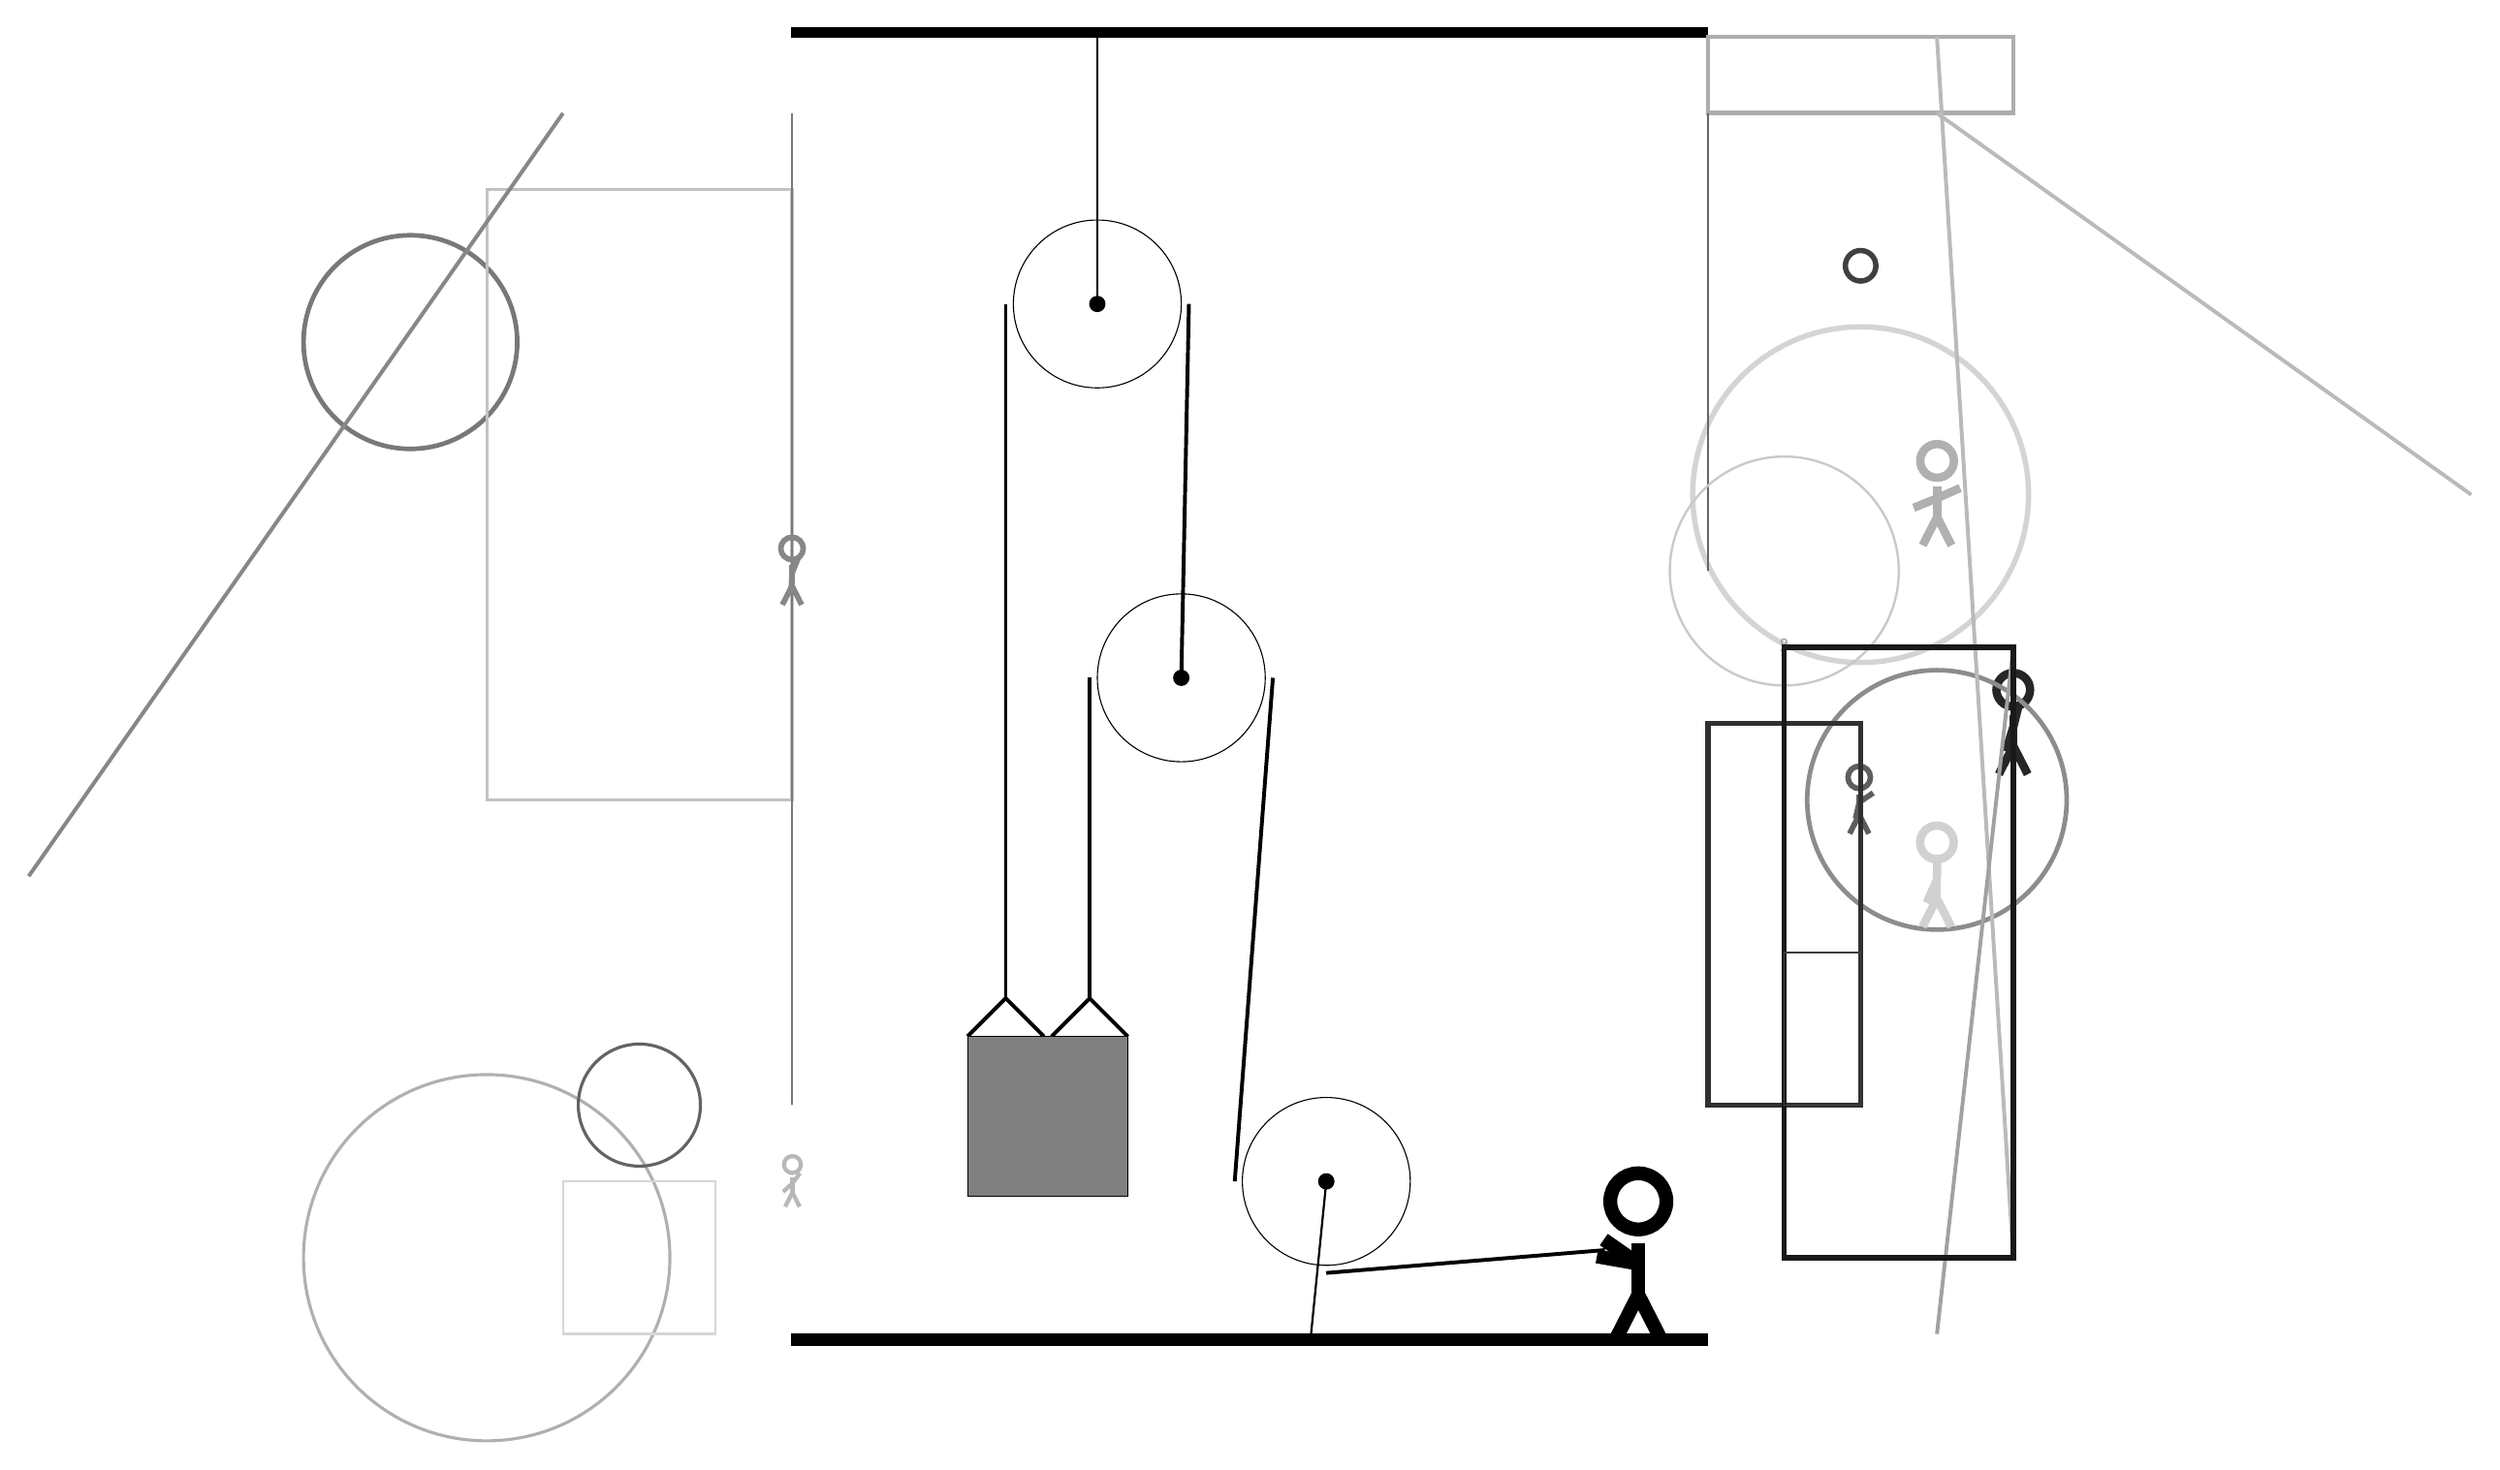
\begin{tikzpicture}
			%%%%% START %%%%%
			
			\draw[fill=black] (-2, 14) rectangle (10, 14.125);
			
			\draw (2, 10.5) circle (1.1);
			\draw[fill=black] (2, 10.5) circle (0.1);
			\draw[thick] (2, 10.5) -- (2, 14);
			
			\node[line width=0.3mm, color=black!85] at (14, 5) {\Strichmaxerl[6][73][76]};
			
			\draw [line width=0.7mm, color=black!17](12, 8) circle (2.2);
			\draw [line width=0.4mm, color=black!31](-6, -2) circle (2.4);
			\draw [line width=0.7mm, color=black!75](12, 11) circle (0.2);
			
			\draw [line width=0.6mm, color=black!45](13, 4) circle (1.7);
			
			\draw [line width=0.6mm, color=black!53](-7, 10) circle (1.4);
			\node[line width=0.6mm, color=black!37] at (11, 6) {\Strichmaxerl[1][39][21]};
			\draw[line width=0.4mm, color=black!24] (-2, 4) rectangle (-6, 12);
			\node[line width=0.6mm, color=black!28] at (-2, -1) {\Strichmaxerl[3][43][53]};
			\draw[line width=0.6mm, color=black!32] (10, 14) rectangle (14, 13);
			\draw[line width=0.5mm, color=black!47](-5, 13) -- (-12, 3);
			\draw[line width=0.5mm, color=black!27](14, -2) -- (13, 14);
			\draw[line width=0.5mm, color=black!27](13, 13) -- (20, 8);
			
			\draw[line width=0.2mm, color=black!52] (-2, 13) rectangle (-2, 0);
			\draw[line width=0.5mm, color=black!37](14, 6) -- (13, -3);
			\draw[line width=0.2mm, color=black!60] (10, 13) rectangle (10, 7);
			
			\node[line width=0.6mm, color=black!31] at (13, 8) {\Strichmaxerl[6][22][24]};
			\draw [line width=0.4mm, color=black!61](-4, 0) circle (0.8);
			\node[line width=0.6mm, color=black!47] at (-2, 7) {\Strichmaxerl[4][87][68]};
			\draw [line width=0.3mm, color=black!21](11, 7) circle (1.5);
			\node[line width=0.4mm, color=black!18] at (13, 3) {\Strichmaxerl[6][66][89]};
			\node[line width=0.3mm, color=black!63] at (12, 4) {\Strichmaxerl[4][77][34]};
			
			\draw[line width=0.7mm, color=black!81] (12, 0) rectangle (10, 5);
			\draw[line width=0.3mm, color=black!16] (-3, -3) rectangle (-5, -1);
			\draw[line width=0.7mm, color=black!90] (11, 6) rectangle (14, -2);
			
			\draw[line width=0.2mm, color=black!76] (12, 0) rectangle (11, 2);
			
			\draw (3.1, 5.6) circle (1.1);
			\draw[fill=black] (3.1, 5.6) circle (0.1);
			
			\draw (5, -1) circle (1.1);
			\draw[fill=black] (5, -1) circle (0.1);
			\draw[thick] (5, -1) -- (4.8, -3);
			
			\draw[line width = 0.5mm]  (0.3, 0.9) -- (0.8, 1.4) -- (1.3, 0.9);
			\draw[line width = 0.5mm]  (1.4, 0.9) -- (1.9, 1.4) -- (2.4, 0.9);
			\draw[fill=black!50] (0.3, 0.9) rectangle (2.4, -1.2);
			
			\draw[line width = 0.5mm] (0.8, 10.5) -- (0.8, 1.4);
			\centerarc[line width = 0.5mm](2, 10.5)(0:180:1.2000000000000002);
			\draw[line width = 0.5mm] (3.2, 10.5) -- (3.1, 5.6);
			\draw[line width = 0.5mm] (1.9, 5.6) -- (1.9, 1.4);
			\centerarc[line width = 0.5mm](3.1, 5.6)(0:180:1.2000000000000002);
			\draw[line width = 0.5mm] (4.3, 5.6) -- (3.8, -1);
			\centerarc[line width = 0.5mm](5, -1)(180:270:1.2000000000000002);
			\draw[line width = 0.5mm] (5, -2.2) -- (8.65, -1.9);
			
			\node at (9, -2) {\Strichmaxerl[10][-35][170]};
			
			\draw[fill=black] (-2, -3) rectangle (10, -3.15);
			
			%%%%% END %%%%%
		\end{tikzpicture}
	\end{figure}	
\end{document}